\documentclass[a4paper,12pt]{foi}

\renewcommand{\brojAutora}{1}

\renewcommand{\naslov}{Aplikacija za analizu velikih količina podataka (NoSQL, map/reduce) - polustrukturirane baze podataka - MongoDB - sa sučeljem na LibreOffice Calc}

\renewcommand{\mentor}{Doc. dr. sc. Markus Schatten} % Ime i prezime mentora

\renewcommand{\autorA}{Tomislav Pertinač}
\renewcommand{\brIndeksaA}{45274/16-R}

\renewcommand{\vrstaRada}{Projektni rad} 

\begin{document}

\maketitle

\tableofcontents

\thispagestyle{empty}

\setcounter{page}{0}

\onehalfspacing

\chapter{Uvod}
U ovome projektu je opisan i prikazan princip rada polustrukturiranih baza podataka, te je prikazano na koji način možemo napraviti i prikazati analizu velikih količina podataka.
Aplikacija za analizu velikih količina podataka je napravljena pomoću NoSQL baze, odnosno korištena je MongoDB baza podataka. Za programski logiku je korišten programski jezik python, a
samo sučelje, odnosno prikaz podataka i analiza je prikazana na LibreOffice tablični kalkulator.\\ 
Aplikacija je funkcionalna na Linux platformi, makar uz malu nadogradnju bi lako bila i funkcionalna na 
Windows platformi. Konretna operacijski sustav koji se koristio za razvijanje aplikacije i na kojem aplikacija radi je Ubuntu 16.04 lts.
U ovom projektnom radu upoznat ćemo se što je to big data i što su polustrukturirane baze podataka. Vidjet ćemo što je to NoSQL po čemu je on različit ili sličan sa SQL-om, bit će opisan MongoDB te će bit prikazana
arhitektura, implementacija te primjer korištenja same aplikacije.

\chapter{Big Data}
Big Data opisuje ogromne količine strukturiranih ili nestrukturiranih podataka s kojima je vrlo teško raditi na klasičan način i korištenjem standardnih alata ili relacijskih baza podataka. Kod big data se često susrećemo sa nazivom V3 odnosno to označava \textit{volume, velocity i variety}. Ponegdje se može još i susreti sa još dvije karakteristike a to su \textit{varijabilnost i vjerodostojnost}.\\
Što se tiče volumena sam naziv big data sve objašnjava. On opisuje ogromnu količinu odnosno volumen podataka koji se tu javljaju.\\
Raznolikost govori o tome da podaci nisu dovoljno strukturirani, da su često neuredni i nabacani iz raznih izvora i na razne načine.\\
Iako se ovdje govori o velikoj količini podataka svejedno nam je važna brzina da  dovoljno brzo i u nekom konačnom, realnom i prihvatljivom vremenu izvučemo za korisnika važne mu podatke koje se kasnije i koriste pri kreiranju izvještaja i za analizu podataka.\\
Pošto se u big data prikupljaju mnogi podaci te se u toj gomili podataka mogu vidjeti realna stanja stvari a to znači i kvalitetu podataka pa zbog toga se negdje i spominje termin vjerodostojnosti u big data.\\
Osim tog termina spominje se još i termin varijabilnosti koji označava da se značenje podataka stalno mijenja. 
U nekim slučajevima čak se zna i naići na još dvije karakteristike. Jedna od njih je vizualizacija gdje je jasno da iz te velike količine podataka se mogu izvući oni bitni i ključni za nekog korisnika, i na temelju njih se mogu raditi analiz i grafovi iz kojih možemo iščitati neke važne inforacije. Te drugi termin je vrijednost, a tu se smatra upravo poslovna vrijednost ili trošak pri korištenju big data tehnologija gdje se važe koliko zapravo korištenje big data tehnologija ima benefita za samo poslovanje.

\chapter{Polustrukturirane baze podataka}
U današnje vrijeme gdje večina svijeta ima pristup internetu, ne čudi da se javila potreba za nekom drugim načinom implementacije baza podataka osim za relacijskim modelom. Tako se zbog sve više korisnika povećava i konstatno obujam podataka koji kruži preko mreže. Tu u igru dolaze polustrukturirani podaci u kojima su informacije sadržane unutar podataka pa se i još znaju zvati "self-describing" ili samo opisne. Polustrukturirani modeli podataka se najčešće prikazuju preko staba. Kod stabla postoji korijen koji predstavlja neki objekt, a vrijednosti se nalaze u svim ostalim birdovima tog stabla.\\
Polustrukturirani podaci su najšeće prikazani pomoću OEM-a odnosno Object exchange modela. Isto tako polustrukturirani podaci su često oblikovani pomoću JSONA ili XML-a. Dok je XML vrlo fleksibilan te ima veliku ulogu u razmjeni raznih podataka na webu, JSON ima prednost što je lakše čitljiv ljudima i jednostavniji računalima za rad sa njim.\\
Kod polustrukturiranih tipova podataka je prednost što objekti ne moraju imati iste atribute, te atributi ne moraju biti isti tip podataka, a samim polustrukturiranim modelom bez problema se mogu prikazati i strukturirani podaci.\\ Neki prednosti i nedostatci su dolje navedeni\\

Prednosti:
\begin{itemize}
\item Programeri koji rade s objektima ne moraju brinuti
o neslaganjima koje prouzročuju objekti
već se s objektima lako manipulira sa light-weight libraryjem.
\item Podrška za ugniježđenim ili hijerarhijskim podacima
pojednostavljuje model podataka koji inače predstavlja složene odnose izmedu entiteta.
\item Podrška za listama objekata pojednostavljuje
model podataka pri čemu se izbjegava nered
konverzije lista u relacijski model podataka.
\end{itemize}

Nedostaci:
\begin{itemize}
\item Tradicionalni model relacijskih podataka
ima popularan i gotov Query Language - SQL.\\
\item Uklanjanjem ograničenja iz modela podataka
sve se manje promišlja da je potrebno razraditi unos podataka.
\end{itemize}

\chapter{NoSQL}
NoSQL baze podataak su baze za pohranu i dohvaćanje podataka koje koriste podosta drugačije principe spram klasičnih relacijskih baza podataka koji koriste tablasti model. NoSQL se još i nazivaju Not Only SQL a se da zaključiti da zapravo podržavaju standradne SQL upite ali i više od toga. Najbitnija razlika je ta da ne koriste Join upite koji su veoma specifični za klasični SQL. Dok spomenemo NoSQL baze podataka tada to povezujemo i sa pojmovima da nisu relacijske, da su distribuirane, otvorenog koda i horizontalno skalabilne.
Što se tiče tipova NoSQL baza podataka, postoji ih nekoliko a to su:
\begin{itemize}
\item Dokumentne baze u kojima se uparuje svaki ključ s kompleksnom podatkovnom strukturom poznatom kao dokument. Dokumenti mogu sadržavati razne parove ključ-vrijednost, parove ključ-polje ili čak i ugniježene dokumente.
\item Grafičke baze se koriste da sačuvaju informacije o nekoj mreži podataka, kao što su na primjer socijalne mreže.
\item Ključ-vrijednost je najjednostavnija NoSQL baza podataka. Svaka pojedina stavka ima ime atributa ili ključ povezanu sa vrijednost.
\item Široko-stupaste baze kao što je npr. Cassandra i HBase su optimizirane za upite nad velikim skupovima podataka. te spremaju stupce podataka zajedno umjesto u redove.
\end{itemize}

NoSQL je odgovor na relacijske baze podataka koje imaju čvrstu strukturu. U današnje vrijeme se sve više koriste agilne metodologije razvoja programskog proizvoda te zbog toga se i često mijenja struktura podataka te tu NoSQL ima prednost jer jednostavnije se nosi sa tim izazovim i zahtjevima. Na slici(\ref{slika-1}). možemo vidjeti ukratko koje su razlike između SQL baza podataka i NoSQL baza podataka.

\begin{figure}[h]
\centering 
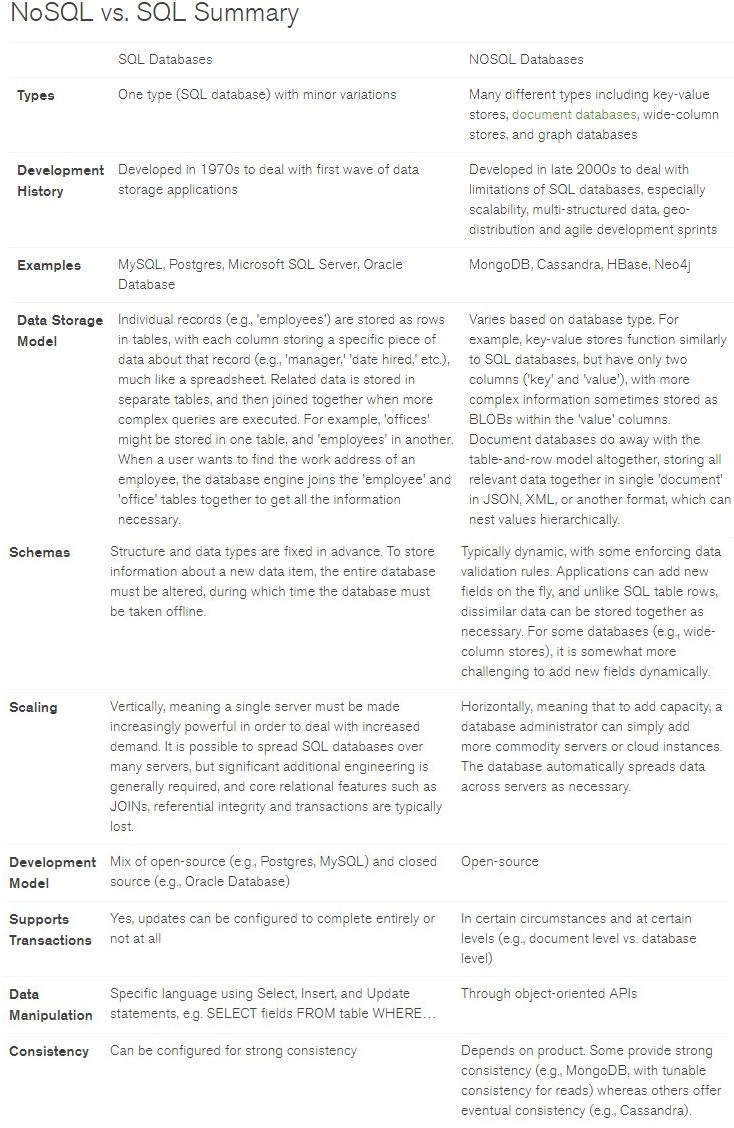
\includegraphics[width=0.95\textwidth]{sql_vs_nosql.jpg}
\caption{SQL vs NoSQL \citep{https://www.mongodb.com/nosql-explained}}
\label{slika-1}
\end{figure}

\chapter{MongoDB}
MongoDB je open-source dokument baza podataka a zapis u MongoDB bazi zove se dokument, koji je podatkovna struktura sastavljena od parova ključeva i njihovih vrijednosti. MongoDB dokumenti su strukturom slični JSON objektima. Vrijednosti polja mogu uključivati i druge dokumente, polja te listu polja.\\
MongoDB sprema BSON dokumente u kolekcije. Što se tiče same razlike u terminologiji kod klasičnih relacijskih baza imamo tablice a to se kod MongoDB-a zovu kolekcije, isto tako redak se zove dokument a stupa je polje.
Rad sa MongoDB-om može ići preko terminala odnosno komadnom linijom ili preko nekih programa za vizualizaciju i olakšano korištenje MongoDB-a kao što je Robomongo. MongoDb ne koristi baš klasične sql upite već pruža neke metode. Tako npr. imamo metode za unos dokumenata u kolekciju(db.collection.insert()), pa za klasičan selekt upit postoji metoda find() nad kojom možemo još i definirat neke dodatne uvjete. Isto tako imamo i metodu update(), delete() te remove(). Postoje i malo specifičnije nabrojene CRUD metode koje se mogu odnosi na samo jedan zapis u kolekciji ili više njih itd.\\
Operacije agregiranja procesiraju zapise podataka i vračaju izračunate rezultate. Takve funkcije obrađuju podatke i prikazuju rezultat u potrebnom obliku. Agregirajuče operacije koriste kolekcije i dokumente kao ulaz i izlaz, poput upita. MongoDB pruža tri načina za izvršavanje agregacije podataka a to su agregacijski cjevovod, map-reduce te agregirajuče funkcije jednostavne svrhe.

\chapter{Izrada baze podataka u MongoDB}
Za početak trebamo skinuti i instalirati MongoDB bazu podataka. Pošto se za operacijski sustav koristi Ubuntu, to ćemo obaviti preko naredba u terminalu i apt sustava za upravljanje paketima.\\
Prvo utipkamo naredbu za uvođenje javnog ključa
\definecolor{lbcolor}{rgb}{0.9,0.9,0.9}
\lstset{commentstyle=\textit,language=python}
\lstset{backgroundcolor=\color{lbcolor},rulecolor=}
\begin{lstlisting}[frame=tb]
sudo apt-key adv --keyserver hkp://keyserver.ubuntu.com:80
--recv 0C49F3730359A14518585931BC711F9BA15703C6
\end{lstlisting}
Zatim kreiramo listu datoteka za Ubuntu verziju koju koristimo, u ovom slučaju je to 16.04
\definecolor{lbcolor}{rgb}{0.9,0.9,0.9}
\lstset{commentstyle=\textit,language=python}
\lstset{backgroundcolor=\color{lbcolor},rulecolor=}
\begin{lstlisting}[frame=tb]
echo "deb [ arch=amd64,arm64 ] 
http://repo.mongodb.org/apt/ubuntu xenial/mongodb-org/3.4 multiverse" 
| sudo tee /etc/apt/sources.list.d/mongodb-org-3.4.list
\end{lstlisting}
Nakon toga učitamo lokalnu bazu podataka paketa
\definecolor{lbcolor}{rgb}{0.9,0.9,0.9}
\lstset{commentstyle=\textit,language=python}
\lstset{backgroundcolor=\color{lbcolor},rulecolor=}
\begin{lstlisting}[frame=tb]
sudo apt-get update
\end{lstlisting}
Sada konačno možemo skinuti i instalirati MongoDB
\definecolor{lbcolor}{rgb}{0.9,0.9,0.9}
\lstset{commentstyle=\textit,language=python}
\lstset{backgroundcolor=\color{lbcolor},rulecolor=}
\begin{lstlisting}[frame=tb]
sudo apt-get install -y mongodb-org
\end{lstlisting}
Nakon što smo to odradili možemo pokrenuti lokalni server sa naredbom
\definecolor{lbcolor}{rgb}{0.9,0.9,0.9}
\lstset{commentstyle=\textit,language=python}
\lstset{backgroundcolor=\color{lbcolor},rulecolor=}
\begin{lstlisting}[frame=tb]
sudo service mongod start
\end{lstlisting}
Naredbe za provjeru statusa servera, resetiranje i zaustavljanje su sljedeće:
\definecolor{lbcolor}{rgb}{0.9,0.9,0.9}
\lstset{commentstyle=\textit,language=python}
\lstset{backgroundcolor=\color{lbcolor},rulecolor=}
\begin{lstlisting}[frame=tb]
sudo service mongod {status|restart|stop}
\end{lstlisting}
Kada bi htjeli nešto testirati i odraditi neke administratorske stvari onda bi utipkali naredbu \textit{mongo} bi nam se tada otvorilo JavaScript shell sučelje za MongoDB.
Za ovu aplikaciju koristimo gotove skupove podataka koji su vezani za rudarenja virtualnih valuta. Tako na slici(\ref{slika-2}) vidimo otprilike kako izgleda model baze u ovoj aplikaciji. 

\begin{figure}[h]
\centering 
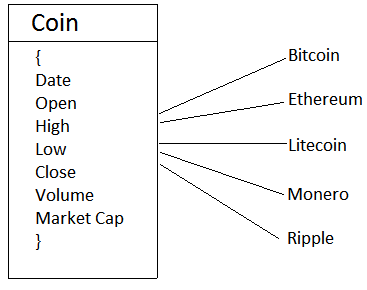
\includegraphics[width=0.95\textwidth]{model.png}
\caption{Model baze}
\label{slika-2}
\end{figure}

Dolje možemo vidjeti dio koda, odnosno JSON-a jednog od kriptovaluta:
\definecolor{lbcolor}{rgb}{0.9,0.9,0.9}
\lstset{commentstyle=\textit,language=python}
\lstset{backgroundcolor=\color{lbcolor},rulecolor=}
\begin{lstlisting}[frame=tb]
{
   "Date": "Aug 15, 2017",
   "Open": 299.95,
   "High": 300.41,
   "Low": 279.33,
   "Close": 289.82,
   "Volume": "1,051,800,000",
   "Market Cap": "28,195,800,000"
 }
\end{lstlisting}

Da konkretnije pojasnimo:
\begin{itemize}
\item Date : datu promatranja
\item Open : Cijena na početku dana
\item High : Najviša cijena u danu
\item Low : Najniža cijena u danu
\item Close : Cijena na kraju danu
\item Volume : Volumen transakcija tog dana
\item Market Cap : Tržišna kapitalizacija u USD
\end{itemize}

Za ovaj projekt smo kreirali novu bazu pod nazivom tbp:
\definecolor{lbcolor}{rgb}{0.9,0.9,0.9}
\lstset{commentstyle=\textit,language=python}
\lstset{backgroundcolor=\color{lbcolor},rulecolor=}
\begin{lstlisting}[frame=tb]
# mongo
> use tbp
\end{lstlisting}
Zatim smo svaki od skupa podataka dodali u bazu:
\definecolor{lbcolor}{rgb}{0.9,0.9,0.9}
\lstset{commentstyle=\textit,language=python}
\lstset{backgroundcolor=\color{lbcolor},rulecolor=}
\begin{lstlisting}[frame=tb]
mongoimport --db tbp --collection bitcoin --file bitcoin.json 
--jsonArray
mongoimport --db tbp --collection ethereum --file ethereum.json 
--jsonArray
mongoimport --db tbp --collection litecoin --file litecoin.json 
--jsonArray
mongoimport --db tbp --collection monero --file monero.json 
--jsonArray
mongoimport --db tbp --collection ripple --file ripple.json 
--jsonArray
\end{lstlisting}

Nakon svih ovih radnji, naša baza je spremna za rad s aplikacijom.

\chapter{Model aplikacije}
Aplikacija u ovom projektu za logiku koristi python programski jezik. Konkretno koristio se PyCharm community ide za lakši razvoj aplikacije. Tako se u pythonu nalazi isprogramirana logika koja se povezuje na MongoDB bazu, radi određene radnji tako da dohvaća određene podake ovisno o upitu te ih zapisuje u LibreOffice te ukoliko odaberemo određene radnje stvara i gafove kroz koje možemo vidjeti neku analizu stanja kriptovaluta(\ref{slika-3}).

\begin{figure}[h]
\centering 
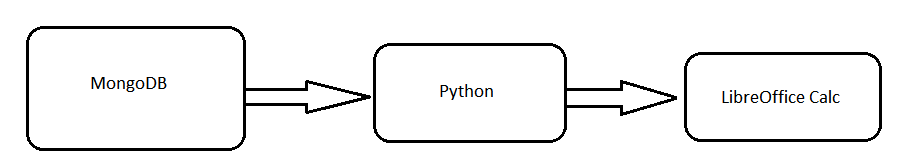
\includegraphics[width=0.95\textwidth]{dizajn.png}
\caption{Model aplikacije}
\label{slika-3}
\end{figure}




















\end{document}